\section{Evaluation}
\label{section:evaluation}
Evaluation of the GearSmarts API was done via Node.js scripts automating the training and classifying of files
stored on the file system. Evaluation was done in two main parts: first evaluating GearSmarts against known, large datasets
to verify the machine learning core works well and as expected, and second evaluating GearSmarts with the collected
outfit-comfort responses.

Evaluations of the classifier are recorded in terms of ``True Positive" (TP), ``False Negative" (FN), ``False Positive"
(FP), \& ``True Negative" (TN), indicating what was predicted versus the data's actual class. Then, the results are
presented in terms of some commonly used formulas: ``Precision", ``Recall", ``Specificity", and ``Accuracy"
\cite{measures}. A description of these formulas is shown in table \ref{table:measures}.

In the case of datasets with more than 2 classes, such as the outfit comfort survey, the measurements are made once for
each of the classes. This shows the performance of the classifier on each class versus all the rest.

\begin{table}
    \begin{tabular}{lll}
        \hline
        \textbf{Measure} & \textbf{Formula} & \textbf{Meaning} \\ [0.5ex]
        \hline\hline
        Precision	& TP / (TP + FP) & \% of correct +'s \\
        Accuracy	& (TP + TN) / (total) & \% correct \\
        Recall 	    & TP / (TP + FN) & \% of +'s predicted as + \\
        Specificity	& TN / (TN + FP) & \% of -'s predicted as + \\
        \hline
    \end{tabular}
    \caption{The measurement terms used in evaluations for this project, with their formulas and intuitive meanings}
    \label{table:measures}
\end{table}

\subsection{Public Datasets}
\label{subsection:publicdatasets}
First, to evaluate the efficacy of the machine learning core, GearSmarts was evaluated using datasets from LIBSVM \cite{libsvm:datasets}.
A large part of the evaluation was the question of how would the feature and classification dictionary and indexing implementation
would impact performance.

A Node.js script was used to parse train and test files, query the GearSmarts API with each, and evaluate the performance.
The evaluation script and datasets can be found in the \texttt{eval/} directory of the source code for this report.
Three public datasets were evaluated: ``a1a'', ``a2a'', and ``a3a'', all with decent results, shown in figure \ref{fig:aXa}.
The datasets have 1,605/30,956, 2,265/30,296, and 3,185/29,376 training/testing datapoints each, respectively.

\begin{figure}[ht!]
    \centering
    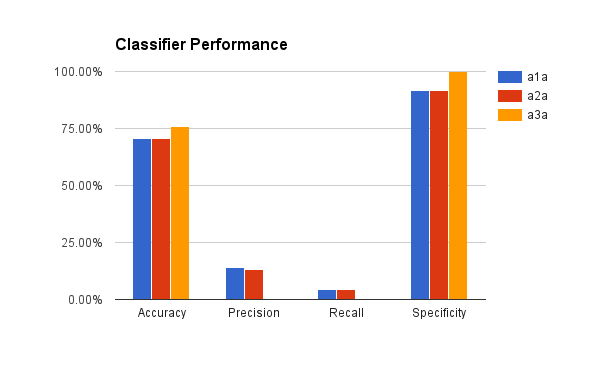
\includegraphics[width=90mm]{img/aXa.png}
    \caption{GearSmarts classifier performance on the aXa datasets}
    \label{fig:aXa}
\end{figure}



\subsection{Outfit Comfort}
In more of an exploration than evaluation, GearSmarts was used to learn and classify the results from a survey on
outfit, activity, and comfort levels. Before evaluating the results, the responses were pre-processed into a normal
form, including weather data from the GearSmarts API.

\subsubsection{Pre-processing}
\label{subsection:preprocessing}
The responses from the survey were transformed in a few phases in order to normalize and extrapolate the information into a
larger, more useful dataset.

The first transformation is from the free-text survey response to a feature-vector CLS structure
containing only a weather link but no data, and activity, demographic, and outfit features. Some interpretation of articles of clothing
was used to reduce the variety of outfit features. Each row in the prepared data
files consists of (1) a class (good, hott, cold), (2) path of the filesystem-cached weather info for that location and
date, and (3) the activity, demographic, and outfit features.

Second, the raw datapoints were duplicated with different classes with the outfit features manually modified to make sense.
This synthesized data is considered reasonable because it followed two rules. The first rule is if someone was hot, adding
more layers will not change the class and vice-versa with removing layers in the cold class. The second rule was more of a
common sense rule to convert ``good'' class rows into ``hott'' and ``cold,'' and convert ``hott'' to ``cold'' class rows
vice-versa. This common sense rule was simply an application of the author's common sense with what it would take to
change someone's comfort level. For example if a skier was ``good`` with the outfit \texttt{[`baseLayerTop', `baseLayerBottom', `fleece', `shell']},
it is reasonable to say they would be made ``hott'' by adding the layers \texttt{[`down',`woolSweater',`sweatPants']}.

Finally, the CSV file was processed to convert each weather directory path into a feature vector which ultimately replaced the
weather path in the data CSV. There was some playing around with which weather features to use, something that will and should
be an ongoing process in the evolution of GearSmarts. Ultimately, only three weather features were used: mean temperature (F),
max wind speed (MPH), and mean dew point (F). These three were selected as their combination roughly provides the metrics
typically seen in weather forecasts: temperature, wind chill, and heat index.

After pre-processing and synthesizing, the comfort dataset consists of 132 datapoints.

\subsubsection{Results}
\label{subsection:preprocessing}
Evaluation of the pre-process comfort was done as for the public datasets, with the additional step of partitioning the
datapoints into training and testing files first. As would be expected for such a small dataset with so many features
(about 12 on average), the results were mediocre; however, they did do better than a dice roll which is an excellent start.
Results for a few random partitions of 60\% training, 40\% testing data are shown in figure \ref{fig:comfort}.

\begin{figure}[ht!]
    \centering
    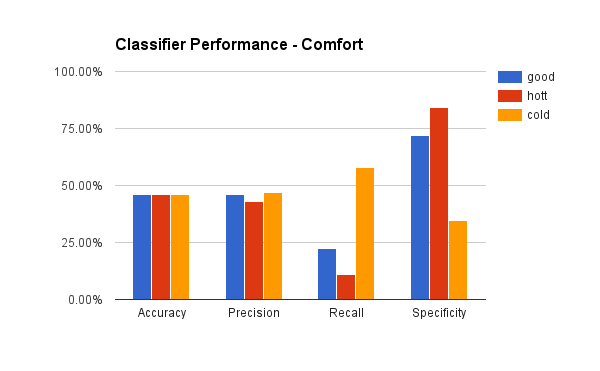
\includegraphics[width=90mm]{img/comfort.png}
    \caption{GearSmarts classifier performance on the outfit comfort dataset, broken up by accuracy against each class}
    \label{fig:comfort}
\end{figure}
